%***** Preamble *****%
\documentclass[a4paper]{article}

%% Language and font encodings
\usepackage[english]{babel}
\usepackage[utf8x]{inputenc}
\usepackage[T1]{fontenc}
\usepackage{graphicx}
\usepackage[font=small,labelfont=bf]{caption}
\usepackage{environ}
\usepackage{amsmath}

%% Sets page size and margins
\usepackage[a4paper,top=3cm,bottom=2cm,left=3cm,right=3cm,marginparwidth=1.75cm]{geometry}

%% Useful packages
\usepackage{amsmath}
\usepackage{graphicx}
\usepackage[colorinlistoftodos]{todonotes}
\usepackage[colorlinks=true, allcolors=blue]{hyperref}

\usepackage{float} % Usado para posicionar imagens
\usepackage{enumitem} % Usado para criar listas enumeradas com letras

\usepackage{listings}
\usepackage{color}
\usepackage{xcolor}

\definecolor{vgreen}{RGB}{104,180,104}
\definecolor{vblue}{RGB}{49,49,255}
\definecolor{vorange}{RGB}{255,143,102}

\lstdefinestyle{verilog-style}
{
    language=Verilog,
    basicstyle=\small\ttfamily,
    keywordstyle=\color{vblue},
    identifierstyle=\color{black},
    commentstyle=\color{vgreen},
    numbers=left,
    numberstyle=\tiny\color{black},
    numbersep=10pt,
    tabsize=4,
    moredelim=*[s][\colorIndex]{[}{]},
    literate=*{:}{:}1
}

\makeatletter
\newcommand*\@lbracket{[}
\newcommand*\@rbracket{]}
\newcommand*\@colon{:}
\newcommand*\colorIndex{%
    \edef\@temp{\the\lst@token}%
    \ifx\@temp\@lbracket \color{black}%
    \else\ifx\@temp\@rbracket \color{black}%
    \else\ifx\@temp\@colon \color{black}%
    \else \color{vorange}%
    \fi\fi\fi
}
\makeatother

\usepackage{trace}


\title{Curso de Verilog - Dia 3}
\author{Caio Rodrigo, Jorge Reis, Manuel Adahil}
\date{} % No Date
%%%%%%%%%%%%%%%%%%%%%%%%%%%%%%%%%%%%%%%%%%%%%%%%%%%%%%%%%%%%%%%%%
%***** Document *****%
\begin{document}
\maketitle

%***** Prática 5 - Behavioral Modelling *****%
\section*{Prática 5 - Behavioral Modelling}

\subsection*{Atividades}
%% Questão 1
\begin{enumerate}
\item Crie um módulo que descreva um Flip-Flop do tipo D ativo em borda de subida e com reset assíncrono e outro com reset síncrono, bem como os seus testbenches.

\begin{figure}[H]
\centering
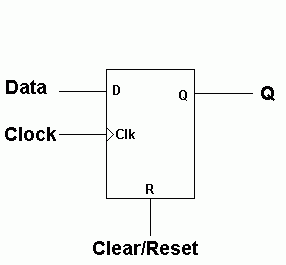
\includegraphics[width=0.3\textwidth]{images/D_FF.png}
\end{figure}

\begin{enumerate}
\item O que acontece em cada um dos casos quando o sinal de Reset é levado ao nível alto e, em seguida, a um nível baixo antes de uma borda de subida do clock?

\item O que foi mudado nos testbenches de cada módulo em relação ao teste do sinal de Reset?

\end{enumerate}
%% Questão 2
\item Crie um módulo que descreva um multiplexador 4x1 em nível comportamental utilizando a estrutura do tipo \textbf{case}(somente o tipo normal). 

\begin{figure}[H]
\centering
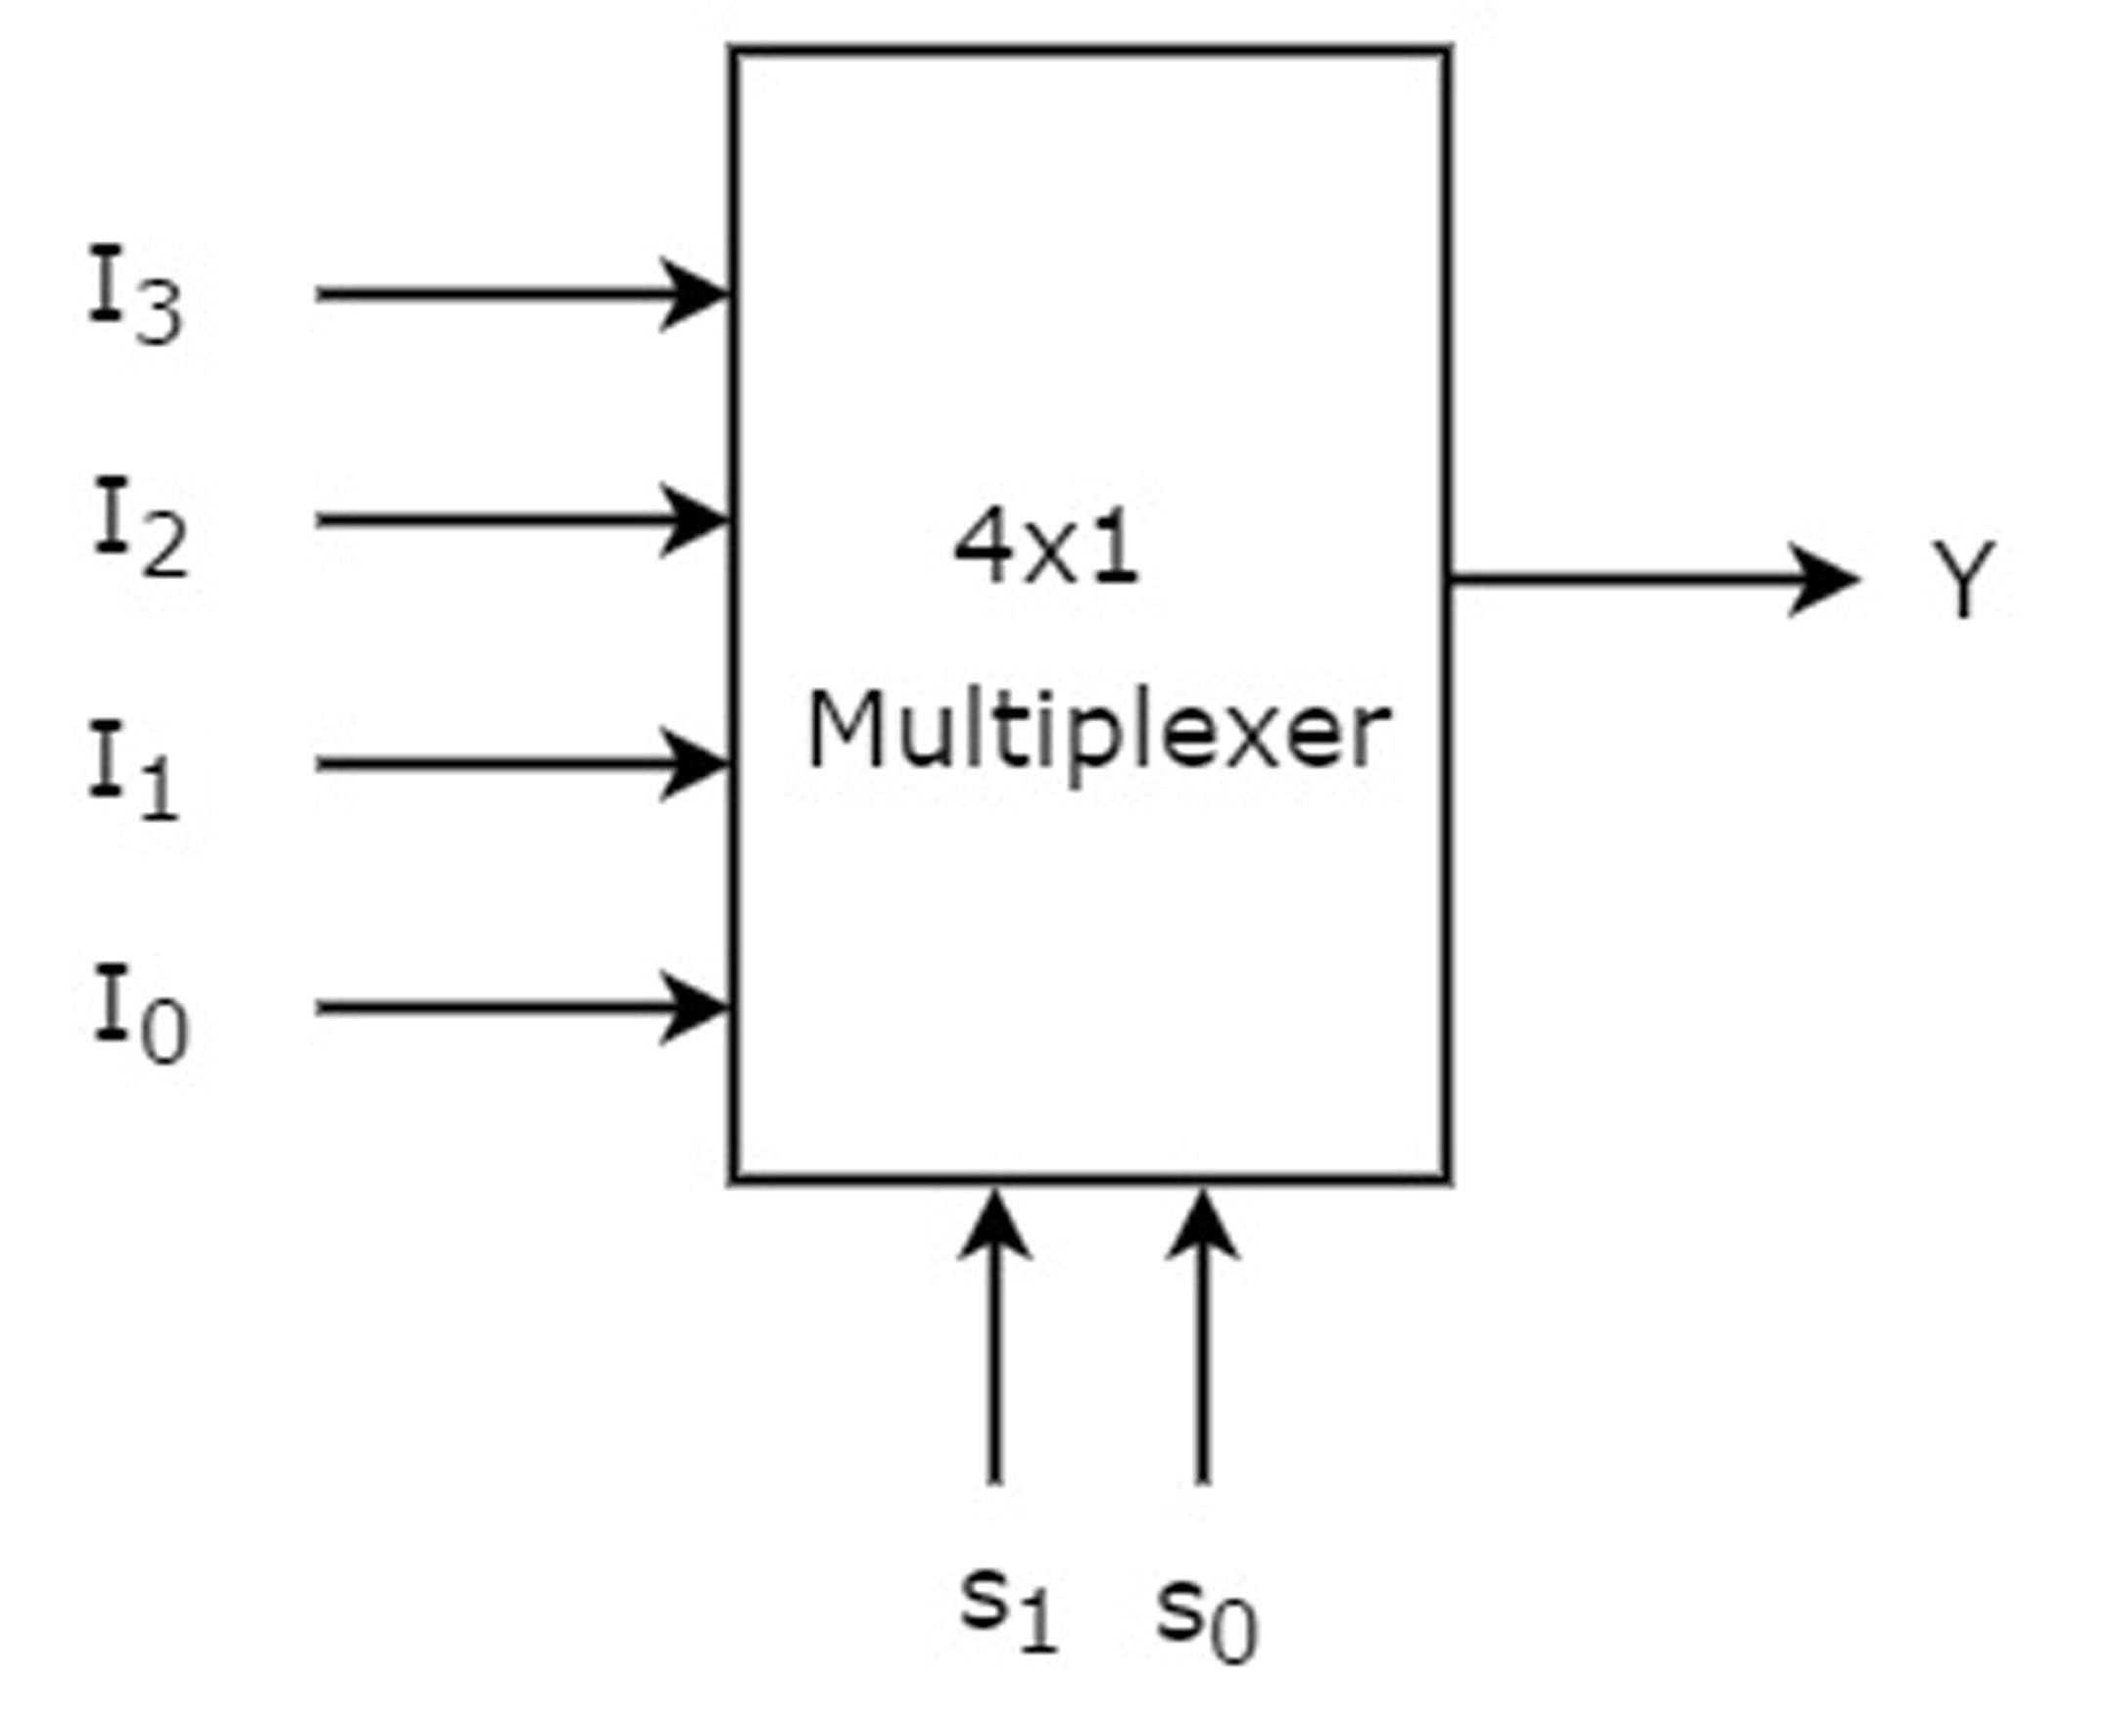
\includegraphics[width=0.3\textwidth]{images/Mux_4x1.png}
\end{figure}

%% Questão 3 - Multiplexador 8x1

\item Desenvolva um multiplexador 8x1, utilizando dois multiplexadores 4x1 e um multiplexador 2X1, bem como seu testbench. Para isso, desenvolva os multiplexadores 4x1 e 2x1 utilizando \textbf{case}.

\end{enumerate}

\subsection*{Fatality}

%% Questão 1 - Register File
Register File é um componente fundamental de qualquer CPU atual pois nele são guardados os registradores (pequenas memórias) que são usadas na execução de instruções de uma CPU. Os registradores são como pequenas variáveis que guardam valores, por exemplo: na instrução \textbf{ADD R3, R1, R2}, os valores de \textbf{R1} e \textbf{R2} são somados e o resultado é escrito em \textbf{R3}.

A estrutura de um register file pode ser vista como no seguinte bloco: 
\begin{figure}[H]
\centering
s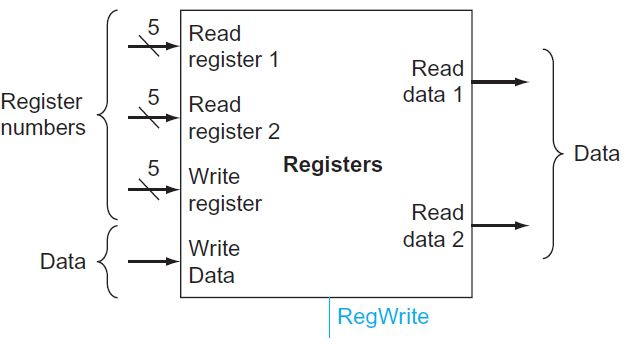
\includegraphics[width=0.4\textwidth]{images/registerfile.jpg}
\caption*{Register File da arquitetura RISC-V.}
\end{figure}
Entradas:
	\begin{itemize}
	\item Read Registers [4:0]: endereço que determina os registradores a serem lidos;
    \item Write Register [4:0]: endereço do registrador a ser escrito;
    \item Write Data [31:0]: Valor a ser escrito no registrador;
    \item RegWrite: habilita o Register File a receber dados pela Write Data;
    \item Clock: sinal omitido na imagem.
	\end{itemize}

Saídas:
	\begin{itemize}
    \item Read Data [31:0]: disponibiliza o valor contido no registrador determinado pelo endereço de Read Register.
    \end{itemize}
    
Crie um Register File de acordo com a arquitetura RISC-V, para isso, leve em conta as seguintes considerações:
	\begin{itemize}
    \item O Register File é um circuito síncrono ativado em borda de subida para realizar operações de escrita e combinacional para realizar operações de leitura, ou seja, a cada borda de subida do clock, é possível fazer uma escrita caso o RegWrite esteja ativo. A leitura poder ser feita a qualquer momento apenas alterando o endereço em Read Register 1 ou 2;
    \item O Register File possui \textbf{32 registradores} de \textbf{32 bits};
    \item A arquitetura RISC-V especifica que qualquer leitura ao endereço registrador zero (\textbf{R0}) deve retornar o valor \textbf{0}.
    \end{itemize}

\end{document}